\section{Technical Experimentation}
In this section, we will present the field we previously described with illustrations. 
\begin{figure}[h!]
    \centering
    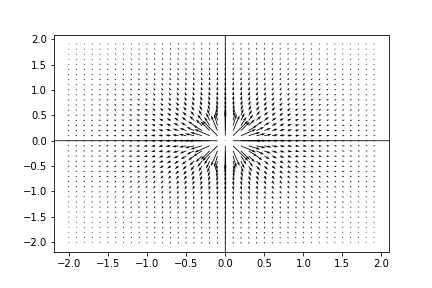
\includegraphics[width=0.48\textwidth]{Images/simplesource.png}
    \caption{Simple Type 1 irrotational source}
    \label{fig:simplesource}
\end{figure}
The field in figure 2 was drawn by computing the gradient of $V_1$ with $(\tilde{{x}_{1}}, \tilde{{x}_{2}}) = (0,0)$ 

\begin{figure}[h!]
    \centering
    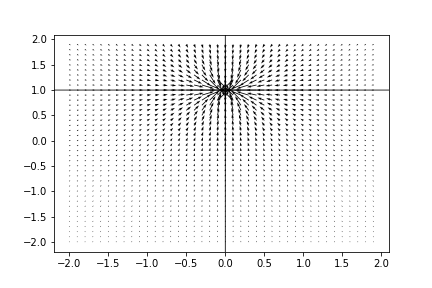
\includegraphics[width=0.48\textwidth]{Images/simplesink01.png}
    \caption{Simple Type 1 irrotational sink}
    \label{fig:simplesink}
\end{figure}
The field in figure 3 is a sink field at $(0,1)$, it is similar to the source field in figure 2 but with opposite sign.

\begin{figure}[h!]
    \centering
    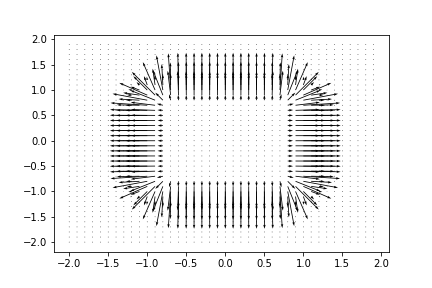
\includegraphics[width=0.48\textwidth]{Images/irrotafromshaping.png}
    \caption{irrotational field from shaping}
    \label{fig:irrotafromshaping}
\end{figure}
The field in figure 4 has been generated by computing the gradient of the shaping function of a superquadratic: 
$F=\frac{1}{1+(\frac{1}{L}H^{\frac{1}{n}})^m}$
As stated in \cite{mcinnes2003velocity}, when $m>>1$ the edge of the shaping function gets more thin and the higher $n$ is the more quadriatic and the less circular the shape will be.

Both these fields are type 1 irrotational solutions of the Laplace equation.

By adding the irrotational sink from figure 3 and the irrotational field from shaping function in figure 4 we obtain a good representation (figure 5) of what the velocity field will look like when close to the target point. 
\begin{figure}[h!]
    \centering
    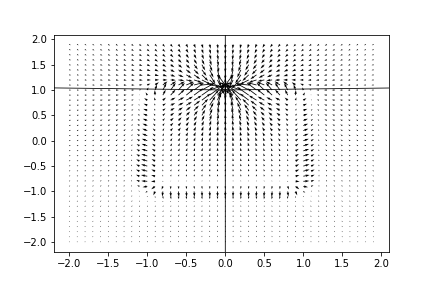
\includegraphics[width=0.48\textwidth]{Images/irrotashapingwithsink.png}
    \caption{irrotational field from shaping with sink}
    \label{fig:irrotafromshapingwithsink}
\end{figure}

The shaping function is mainly used to generate a vortex field around an obstacle, as explained in the paper, it is given by: 
$v_2=-\frac{\partial{F}}{\partial{x_2}}e_1 + \frac{\partial{F}}{\partial{x_1}}e_2 $
We can see in figure 5 an example of vortex field around a super quadriatic
\begin{figure}[h!]
    \centering
    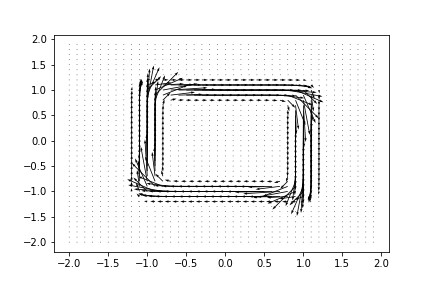
\includegraphics[width=0.48\textwidth]{Images/rotafromshaping.png}
    \caption{Solenoidale field from shaping function}
    \label{fig:rotafromshaping}
\end{figure}

As explained in section 2, after we made contact, we stop using the potential based field and we use the spherical field to maintain 
contact with the desired force. 
Figure 6 represents an example of such a field: 
\begin{figure}[h!]
    \centering
    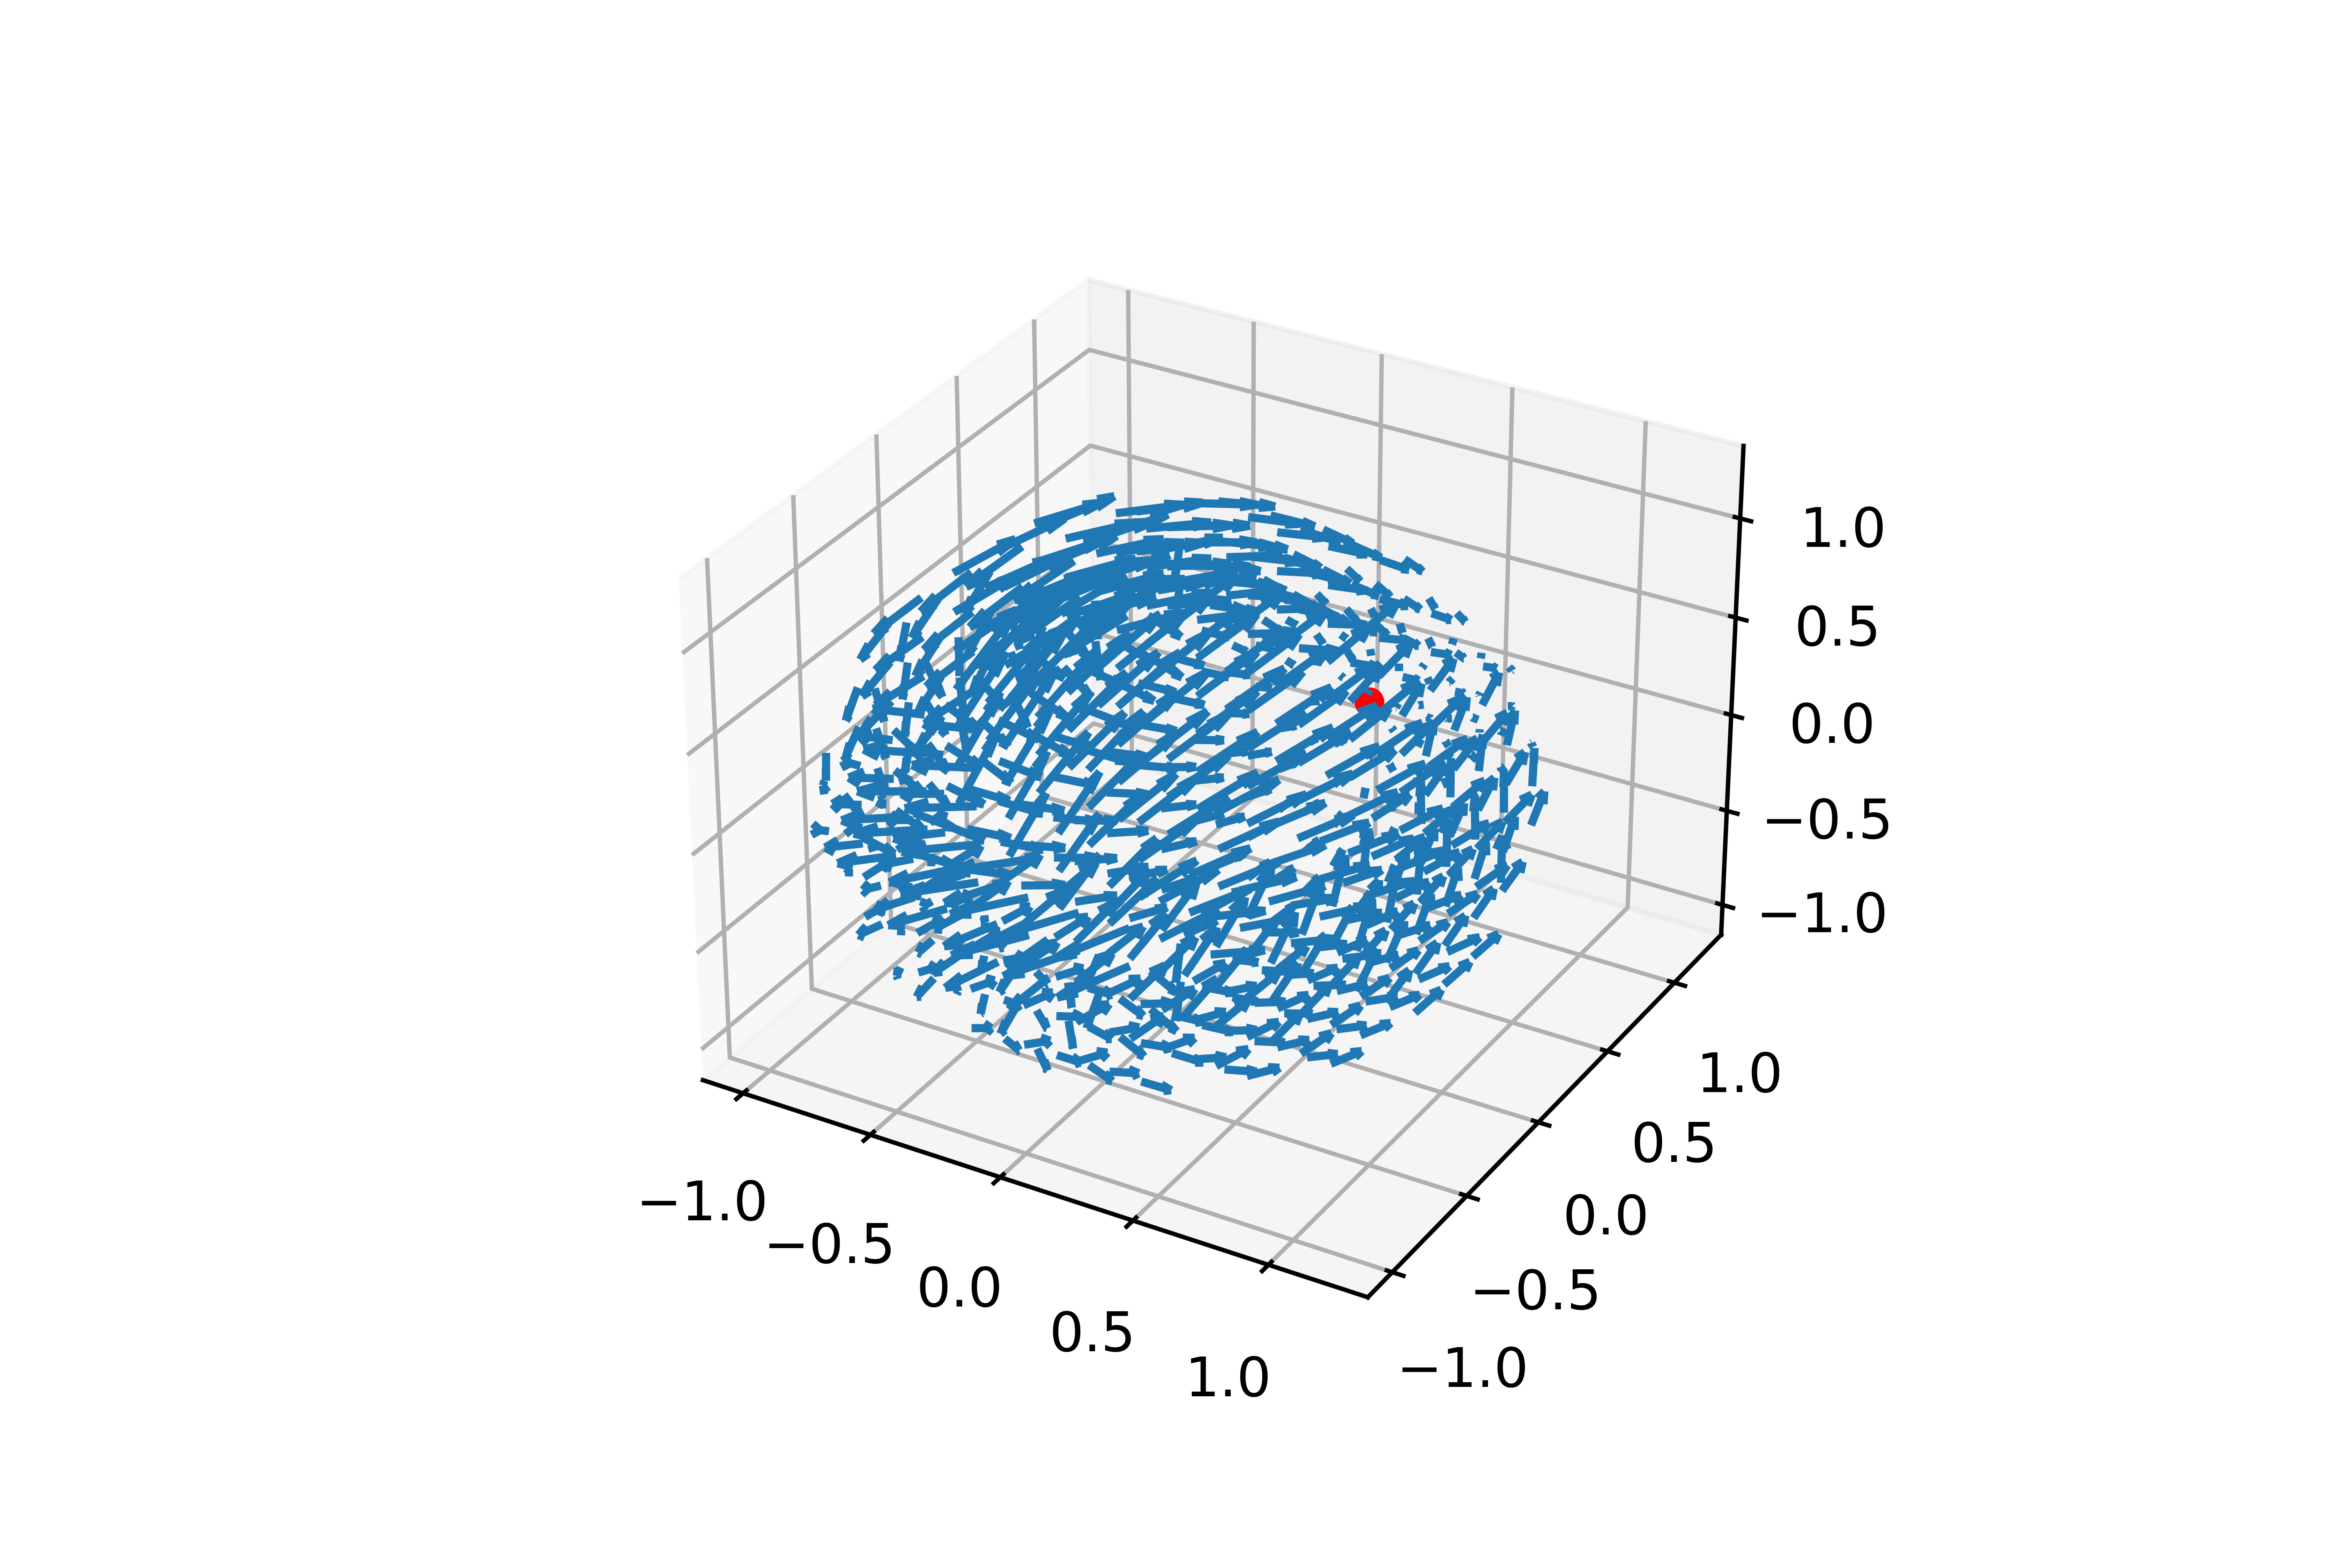
\includegraphics[width=0.48\textwidth]{Images/sphericalfield.png}
    \caption{Spherical contact field}
    \label{fig:spherical}
\end{figure}
